\documentclass[10pt,xcolor=x11names,compress, notes=show]{beamer}% pour l'impression, tout n'apparait qu'une fois \documentclass[handout,12pt]{beamer}

%\documentclass[xcolor=x11names]{beamer}
%\usepackage[scaled]{helvet}
\usepackage[round]{natbib}



\usepackage[utf8x]{inputenc}
\usepackage{ucs}
\usepackage[french]{babel}
\usepackage{todonotes}
\usepackage{tikz}
\usepackage{color}
%\usepackage{subfigure}
%\usepackage[]{geometry}
\usepackage{changepage}
\usetikzlibrary{calc}

\usepackage{bm}
\usepackage{pifont} %pour les symbole sympa \ding{nb}
\usepackage[export]{adjustbox}
\usepackage{subcaption}


\setbeamertemplate{navigation symbols}{} 


%\usepackage{palatino}

%pour le theme
%\usetheme{CambridgeUS}

%\usetheme{Goettingen}
\useinnertheme{default}
\useoutertheme[subsection=false]{miniframes}
\setbeamertemplate{blocks}[rounded][shadow=true]
\setbeamercolor{block title}{fg=DeepSkyBlue4,bg=DeepSkyBlue4!10}
\setbeamercolor{block title alerted}{bg=DeepSkyBlue4!0} 
\setbeamercolor{block title example}{bg=DeepSkyBlue4!20}
\setbeamercolor*{lower separation line head}{bg=DeepSkyBlue4} 

\setbeamerfont{title like}{shape=\scshape}
\setbeamercolor{frametitle}{fg=DeepSkyBlue4}
\setbeamercolor{title}{fg=DeepSkyBlue4}
\setbeamercolor{itemize item}{fg=black}
\setbeamercolor{itemize subitem}{fg=black}
\setbeamercolor{toc}{fg=DeepSkyBlue4}
\usepackage{amsmath,mathtools}
\usefonttheme[onlymath]{serif}

\setbeamertemplate{frametitle}{\vspace{0.13cm}\hspace{-0.9cm} \insertframetitle}
\setbeamerfont{frametitle}{size=\Large}

\setlength{\fboxrule}{1pt}

\setbeamertemplate{bibliography item}[]

%couleur table des matières
\usepackage{hyperref}
\hypersetup{colorlinks=true, linkcolor=DeepSkyBlue4}

\setbeamertemplate{caption}{\raggedright\insertcaption\par}

%Mettre la section courante en titre de diapo (pour champ de titre non-vide)
%\addtobeamertemplate{frametitle}{\frametitle{\insertsubsectionhead}}{}

\addtobeamertemplate{footline}{\hspace{11cm} \insertframenumber/\inserttotalframenumber}

\newcommand{\tr}[1]{\prescript{t\hspace{-0.08cm}}{}{#1}}



%page de titre
\author{Alice \textsc{Dinsenmeyer} \\~\\ encadrée par\\ Romain \textsc{Brossier} \& Ludovic \textsc{Moreau} \\ Maîtres de conférences, ISTerre}

\title{Imagerie ultrasonore par inversion de formes d'onde}
\subtitle{}
\date{\small 12 juillet 2016}

\titlegraphic{
\begin{minipage}{0.3\textwidth}
	\centering
	\includegraphics[height=1cm]{img/univ.png}	
\end{minipage}
\begin{minipage}{0.3\textwidth}
	\centering	
	\includegraphics[height=1cm]{img/cnrs.png}
\end{minipage}
\begin{minipage}{0.3\textwidth}
	\centering
	\includegraphics[height=1cm]{img/isterre.png}
\end{minipage}

}


\begin{document}

\begin{frame}
	\titlepage 
\end{frame}



\begin{frame}
\setlength{\leftmargin}{-2cm}
\setlength{\rightmargin}{-2cm}
%\setlength{\textwidth}{29cm}
\begin{picture}(0,0)(0,0)\put(-20,-180){
	$v_{p}$
}\end{picture}
\begin{picture}(0,0)(0,0)\put(-20,-180){
	$\rho$
}\end{picture}
	\begin{columns}
		\column{0.3\textwidth}
		\centering
		\small{Initial \\ model}
		\includegraphics[height=1.9cm]{img/vp_mono_smooth/vp_smooth.png}\\
		
\includegraphics[height=1.9cm]{img/rho_mono/rho_init.png}		
		\column{0.3\textwidth}
		\centering
		\small{Monoparameter inversion}
		\includegraphics[height=1.9cm]{img/vp_mono_uni/vp_3300k.png}\\
		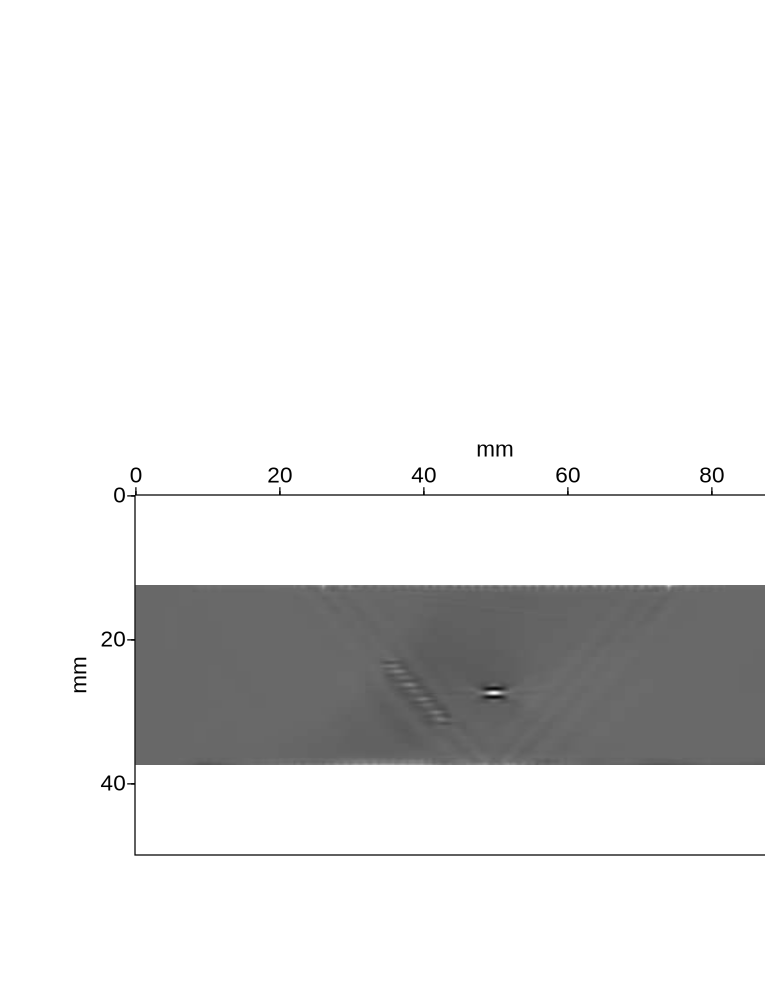
\includegraphics[height=1.9cm]{img/rho_mono/rho_mono.png}		
		\column{0.3\textwidth}
		\centering
		\small{Multiparameter inversion}
		\includegraphics[height=1.9cm]{img/multi/vp_multi_6000k.png}\\		
		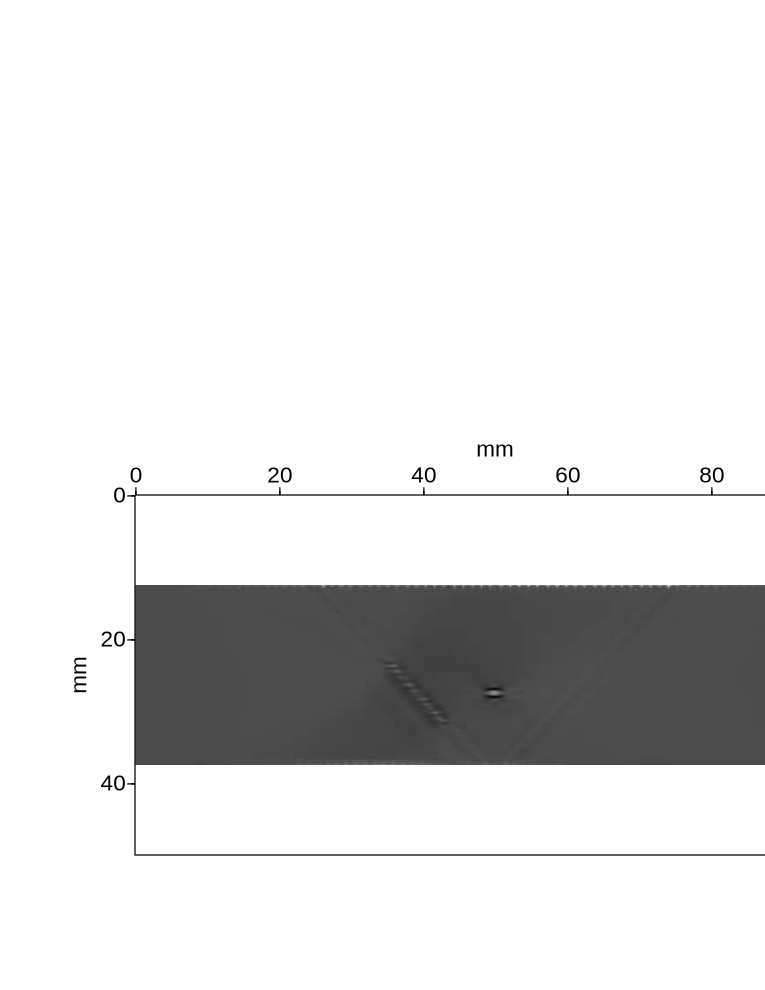
\includegraphics[height=1.9cm]{img/multi/rho_6000k.png}\\		
	\end{columns}
\end{frame}


\end{document}
